\subsubsection{Conceptual Data Schema}

The system's conceptual data schema is presented in Figure \ref{fig:conceptual-data-schema}. It includes the main domain entities (classes), their essential properties (attributes), and the relationships among them (associations, aggregations, compositions, and generalizations).

\begin{figure}[H]
    \centering
    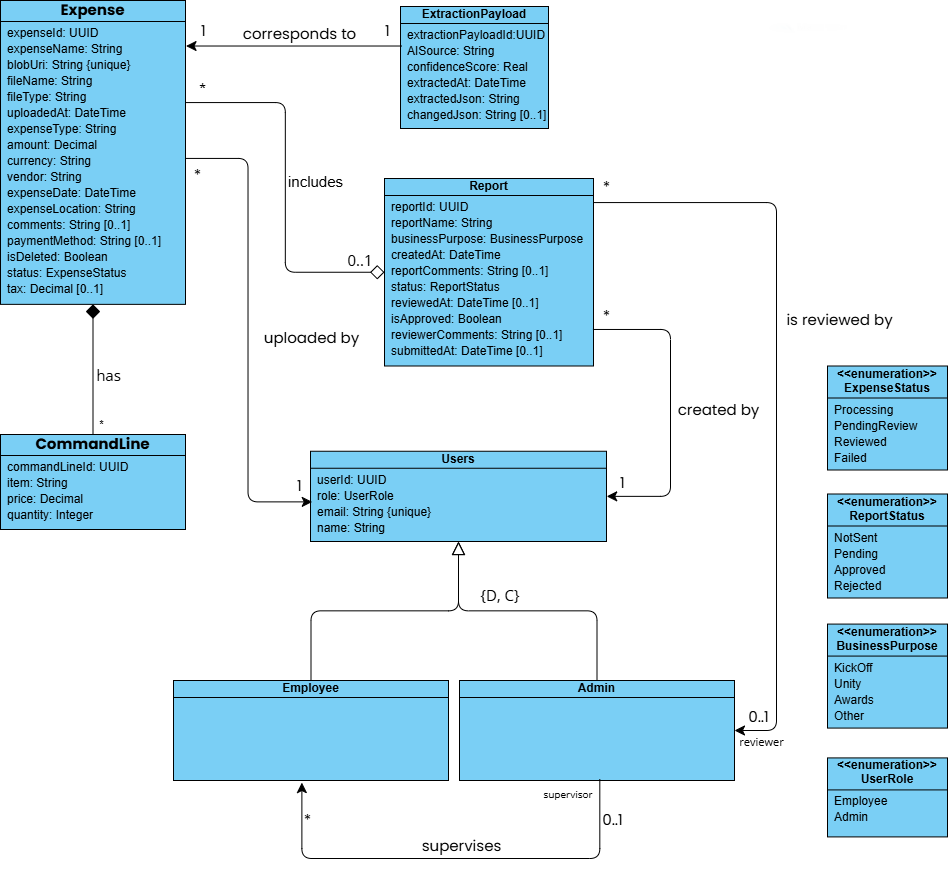
\includegraphics[width=\textwidth]{Images/UML.png}
    \caption[Conceptual data schema]
    {Conceptual data schema. [Own creation]}
    \label{fig:conceptual-data-schema}
\end{figure}

\newpage

